\documentclass[10.5pt,border={10pt 10pt 10pt 10pt}]{standalone}
\usepackage{tikz}
\usepackage{amsmath}
\usetikzlibrary{shapes.misc, positioning}
\usetikzlibrary{fit,positioning}

\usepackage{xcolor}
\definecolor{col}{RGB}{31,64,122}

\begin{document}
\centering
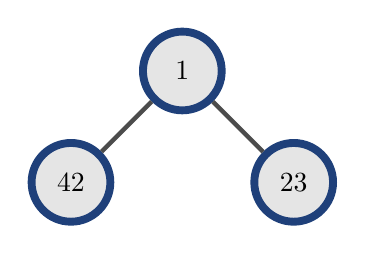
\begin{tikzpicture}
	\tikzset{
		ellipse/.style={%
           	draw,                 
	         shape=circle,
              line width=1mm,
             inner sep=0pt,        
             node distance=2cm,
             minimum size=10mm}
       } 
       

       \tikzstyle{edge_style} = [draw=black!70, line width=2, ultra thick]         
	
	  \node[ellipse,draw=col, fill=black!10] (a) at (0, 0)  {$1$};
	  \node[ellipse,draw=col, below right of= a, fill=black!10] (b) {$23$};
	  \node[ellipse,draw=col, below left of= a, fill=black!10] (c) {$42$};

	
	  \draw[edge_style]  (a) edge (b);
	  \draw[edge_style]  (c) edge (a);

\end{tikzpicture}

\end{document}